Figure \ref{fig:images-q6a} shows all paths for the modified 4-node network
problem, containing the following paths:

\begin{align*}
	\mathbb{P}_1 = \{P_{1,1}1,P_{1,2},P_{1,3}\} &= \{\{2,4\},\{1,5\},\{4,3,1\}\} \\
	\mathbb{P}_2 = \{P_{2,1},P_{2,2}\} &= \{\{5\},\{4,3\}\} \\
	\mathbb{P}_3 = \{P_{3,1},P_{3,2}\} &= \{\{1\},\{3,2\}\}
.\end{align*}

\begin{figure}[H]
	\centering
	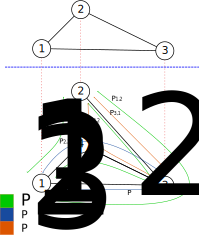
\includegraphics[width=0.8\textwidth]{images/q6a}
	\caption{Paths for Question 6 Part a}
	\label{fig:images-q6a}
\end{figure}
